
\documentclass{beamer}
\usepackage{ucs}
\usepackage[utf8x]{inputenc}
%\usepackage[T1]{fontenc}

\usepackage{graphicx}
\usepackage{tipa}
\usepackage{multirow}
\usepackage{tabularx} %specified width

\begin{document}
\title{OAHPA -- pedagogical programs based on linguistic resources}   
\author{Lene Antonsen, University of Tromsø 
\begin{figure}  \scalebox{0.10}[0.10]{
\includegraphics{img/LogoSamisk}} \end{figure}} 
\date{} 


\frame{\titlepage} 
\frame{\frametitle{Project}
\textbf{teamwork:}\\
Lene Antonsen, Biret Ánne Bals Baal, \\ Saara Huhmarniemi, Trond Trosterud, Kjellaug Isaksen \\
\vspace{0.5cm}
\textbf{with grants from:}\\
\begin{itemize}
\item Faculty of Humanities at the University of Tromsø \item Sámi Parliament in Norway
\item Research Council of Norway has financed the work behind the basic analysers
\end{itemize}
}

\frame{\frametitle{Our analysers}
\begin{itemize}
\item a pre-processor for sentence boundary detection and tokenization.\\ 
- abbreviations, - multi-word expressions
\item a morphological analyser with finite state transducers, compiled with the Xerox compiler xfst. \\ - lexical transducer for morphology lexc,  phonological transducer, twolc.  sme: 97.500 lemmas  
\item an interface to the morphological analyser, lookup. 
\item a morphological disambiguator based on constraint grammar with manually written rule sets (vislcg3). sme: 3300 rules
\end{itemize}
} 

\frame{\frametitle{The pedagogical idea}

\begin{itemize}
\item Flexibility -- choose what to exercise
\item Possibility of restricting the vocabulary to particular textbooks
\item Choose topics instead of textbooks
\item Choose between the main dialects for the task
\item Immediately feedback about errors
\item Get translation and grammar help easily
\item Accessible freely via Internet, without installing new programs in the computer
\end{itemize}
} 


\frame{\frametitle{Lexicon}
Example of entry in the main lexicon.\\ AIGI is the continuation class. \\
\vspace{0.5cm}
\scalebox{.8}[.8]{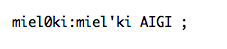
\includegraphics{img/noun-sme-lex.png}}\\
}

\frame{\frametitle{Entry in the pedagogical lexicon}
\scalebox{.55}[.55]{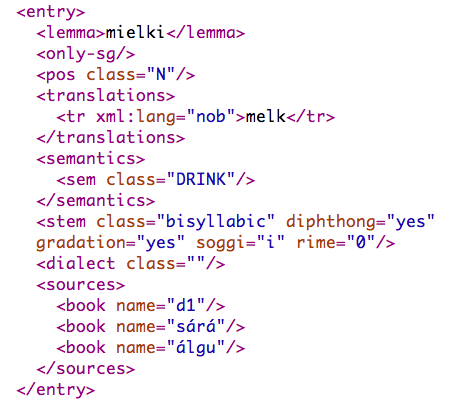
\includegraphics{img/nounlexicon.png}}
}

\frame{\frametitle{Homonomies}
\begin{itemize}
\item \textit{girdi}: "plane" (VEHICLE) or "pilot" (PROFESSION) 
\item \textit{bassi} Sg -- \textit{basit} Pl (= holy day) and \textit{bassi} Sg -- \textit{bassit} Pl (= washer).
\end{itemize}
\vspace{0.5cm}
Solution: \\
\texttt{id="girdi\_vehicle"} vs. 
\texttt{id="girdi\_profession"} \\ \texttt{id="bassi\_time"} vs. \texttt{id="bassi\_actor"}.
}

\frame{\frametitle{Sentence generator}
\scalebox{.6}[.6]{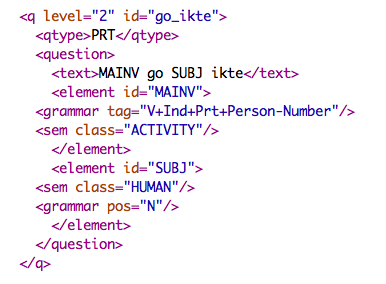
\includegraphics{img/question_vasta.png}}
}


\frame{\frametitle{Semantic sets}
Some of the semantic sets are supersets, consisting of subsets. 
\vspace{0.5cm}

\scalebox{.6}[.6]{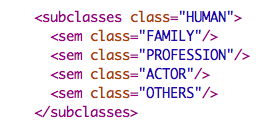
\includegraphics{img/semantic_set.png}}
}

\frame{\frametitle{Generating question and answer pairs}
QPN - question's person-number \\
APN - answer's person-number\\
\vspace{0.5cm}
\begin{tabular}[t]{ll|ll|ll}
QPN &APN &QPN &APN &QPN &APN \\
\hline
Sg1 &Sg2 &Du1 &Du2 &Pl1 &Pl2 \\
Sg2 &Sg1 &Du2 &Du1 &Pl2 &Pl1 \\
Sg3 &Sg3 &Du3 &Du3 &Pl3 &Pl3 \\
\hline
\end{tabular}
}

\frame{\frametitle{System for dialectical variation}
Marked both in lexicon and in the morphology files:
\vspace{0.3cm}
\begin {itemize}
\item \^{}NG\^{}  (not generate for any of the dialects)
\item NOT-KJ (not generate for KJ-dialect) 
\item NOT-GG (not generate for GG-dialect)  
\end {itemize}
\scalebox{.6}[.6]{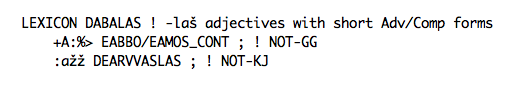
\includegraphics{img/smelex.png}}\\
In the makefile there are options to generate the chosen dialectical variants of word forms, for the \texttt{strict-sme.fst} .
}

\frame{\frametitle{System for feedback on morphology}
\scalebox{.7}[.7]{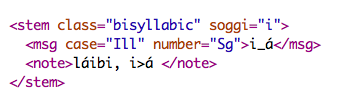
\includegraphics{img/feedback_nouns.png}}\\
The features in the lexicon are used to give message tags. 

\scalebox{.7}[.7]{
\includegraphics{img/messages.png}}\\
Feedback to the student's is generated from the message tags. 
}


\frame{\frametitle{Student's input}
Acceptable answers:\\
\textit{Maid don lohket ikte?} (What did you read yesterday?)
\begin{itemize}
\item \textit{Mun han lohken ollu áviissaid.} (I PART read many newspapers.)
\item \textit{Ikte mun gal lohken buori girjji.} (Yesterday I PART read a good book.)
\item \textit{In lohkan maidege.} (I did not read anything.)
\item \textit{Ikte in lohkan.} (Yesterday I did not read.)
\end{itemize}
}

\frame{\frametitle{Feedback to student}
The Vasta-program gives feedback if the answer is not acceptable:
\begin{itemize}
\item \textit{Mun lohket ollu áviissaid.} \\ $\rightarrow$ Remember agreement between subject and verbal.  
\item \textit{Mun lohken ollu áviissat.} \\ $\rightarrow$ There should be an accusative in your answer. 
\item \textit{Don lohket ollu áviissaid.} \\ $\rightarrow$ Are you sure that you answer in the correct person?  
\end{itemize}
}


\frame{\frametitle{Analyser for student's input}
\scalebox{.31}[.31]{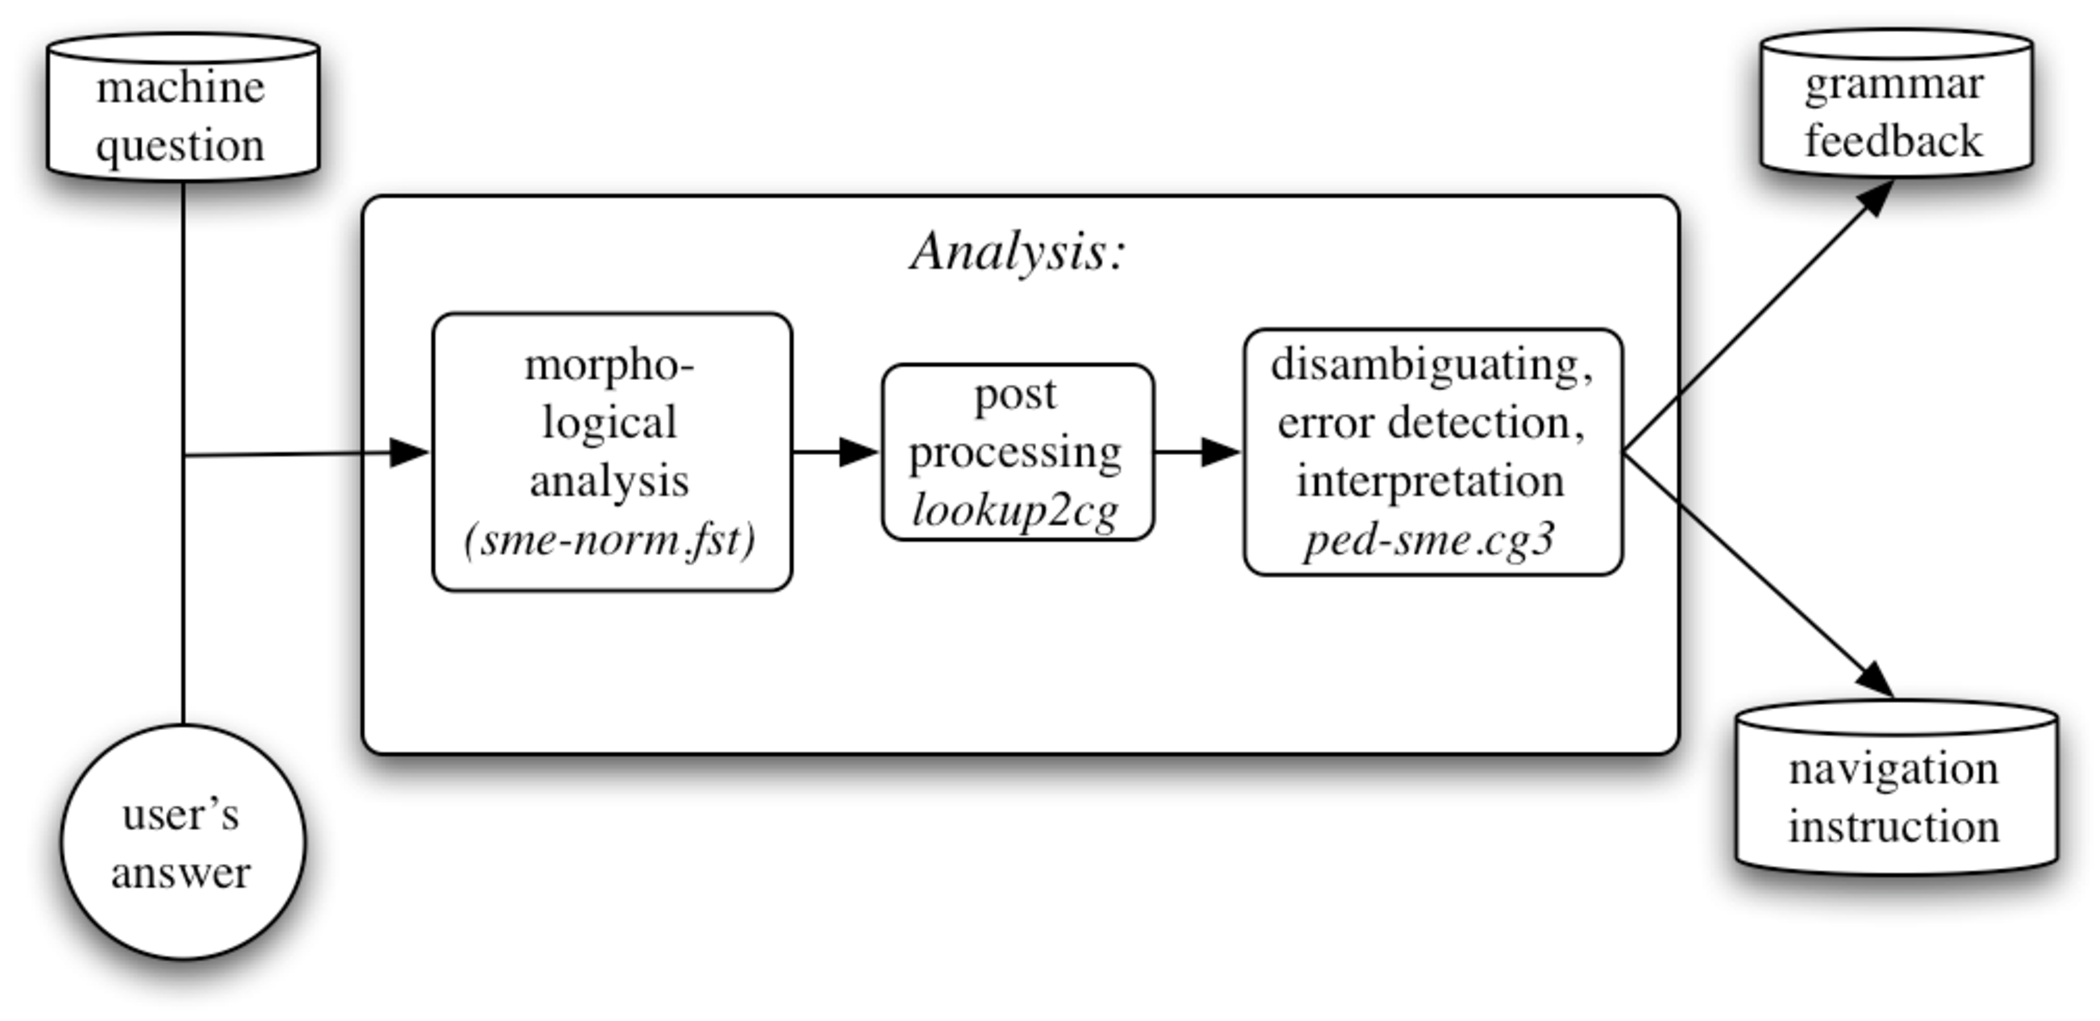
\includegraphics{img/qa.pdf}}
}

\frame{\frametitle{Analysis of student's input, before disambiguation}
\scalebox{.45}[.45]{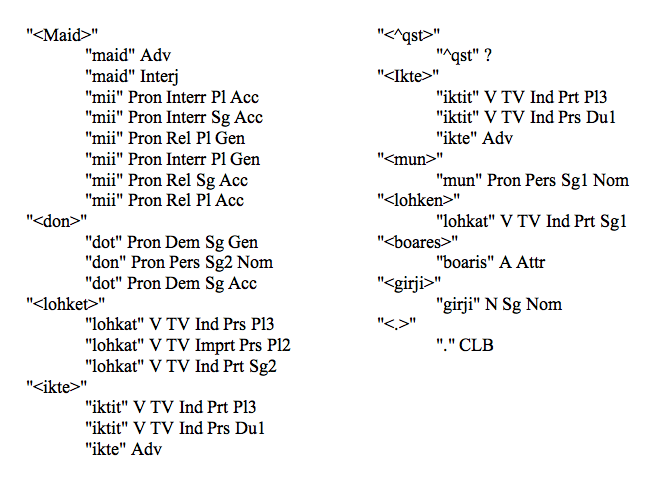
\includegraphics{img/iktelohken2.png}}\\
What did you read yesterday? Yesterday I read an old book (Nom instead of Acc)
}

\frame{\frametitle{Finding the case error with constraint grammar}
\scalebox{.56}[.56]{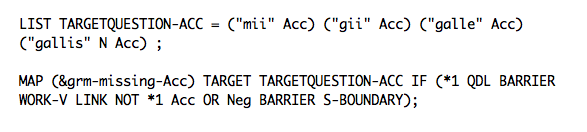
\includegraphics{img/pedcg3.png}}\\
If the interrogative pronoun is in accusative, we expect an accusative or a negation in the answer\\
- if  not asking for a verb, e.g. "What do you do?" (WORK-V). }

\frame{\frametitle{Analysis after disambiguation}
\scalebox{.5}[.5]{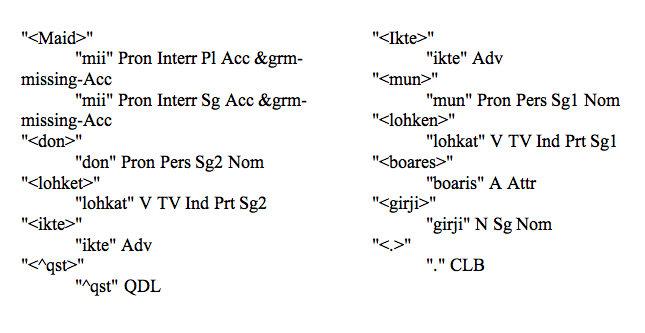
\includegraphics{img/maid_lohket_ikte2.png}}\\
The grammarerrortag (\&grm-missing-Acc) is added to the interrogative pronoun. }


\frame{\frametitle{Tutorial feedback}
\scalebox{.5}[.5]{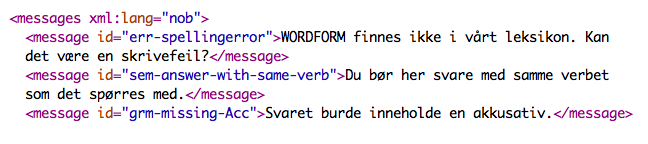
\includegraphics{img/messages_vasta.png}}\\
The grammarerrortag generates tutorial feedback, which can be generated in different languages. nob = Norwegian.
}

\frame{\frametitle{Errors in input}
There can be misspellings or that the student does not know the correct inflection.
\begin{itemize}
\item notexisting word \\ $\rightarrow$ Feedback: The word is not in the lexicon, can it be a misspelling? 
\item correct lemma, unintended wordform \\ $\rightarrow$ Feedback made from the context
\item unintended lemma \\ $\rightarrow$ Feedback has to be tailored from what we know about the student's interlanguage -- and we make rules for typical unintended lemmas
\end{itemize}
}



\frame{\frametitle{Navigating in the dialogue}
\scalebox{.55}[.55]{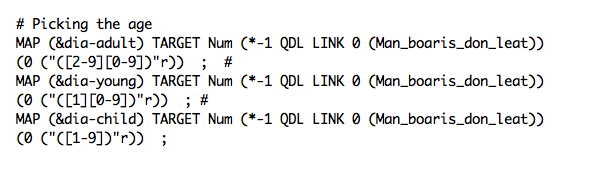
\includegraphics{img/picking_age.png}}\\
Rules for giving age-tag to the input. \\ These are special rules for the question named Man\_boaris\_don\_leat (How\_old\_are\_you).}

\frame{\frametitle{Navigating in the dialogue}
\scalebox{.6}[.6]{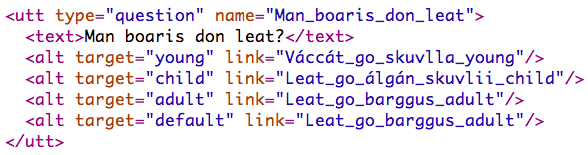
\includegraphics{img/Man_boaris.png}}\\
Navigating to the next question or branch, with help of the tag. \\The branches are adapted to the age of the student. }

\frame{\frametitle{Navigating in the dialogue}
\scalebox{.6}[.6]{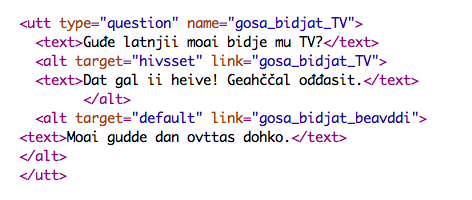
\includegraphics{img/gosabidjatTV.png}}\\
"To which room we put the TV?" \\ 
If the student answer with "hivsset" ( = WC), the answer is "It is not a good idea. Make a new try." \\
Default is: "We carry it there together." }


\frame{\frametitle{Navigating in the dialogue}
\scalebox{.58}[.58]{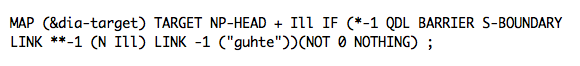
\includegraphics{img/targetIll.png}}\\
Map \&dia-target to the NP-head in illative after a question\\ with the interrogate \textit{guhte} + a noun in illative ( = "to which N"),\\ if the answer isn't "not anywhere".}


\frame{\frametitle{OAHPA-programs}
\textit{http://victorio.uit.no/oahpa/}
\begin{itemize}
\item  \textbf{Numra}: Exercise numerals
\item \textbf{Leksa}: Sátnequiz - Sámi/Norwegian and Norwegian/Sámi
\item  \textbf{Morfa}: Exercise word inflection, also in context
\item  \textbf{Vasta}: Exercise answering to questions
\item  \textbf{Sahka}: Participate in dialogues
\end{itemize}
}

\frame{\frametitle{Numra -- numeral exercise}
\scalebox{.5}[.5]{
\includegraphics{img/numra.png}}
}

\frame{\frametitle{Leksa -- word quiz}
\scalebox{.5}[.5]{
\includegraphics{img/leksa.png}}
}

\frame{\frametitle{Morfa-S -- word inflection}
\scalebox{.45}[.45]{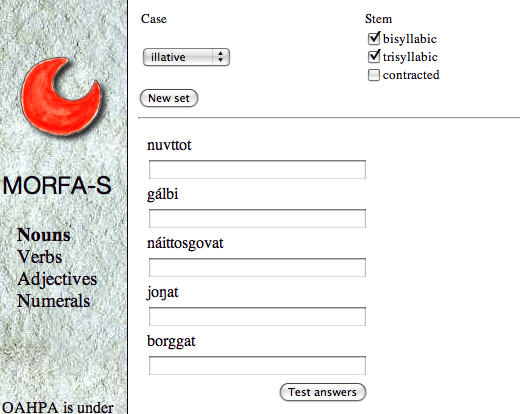
\includegraphics{img/morfaS.png}}
}

%\frame{\frametitle{Morfa S -- tasks}
%\begin{itemize}
%\item Nouns: nominative pl and all oblique cases (sg and pl mixed). Also some place names.
%\item Verbs: indicative present tense, indicative past tense, conditional, potentional, imperative
%\item Adjectives: attributive, nominative pl and all other cases (with sg and pl mixed). For all one can choose a grade: positive, comparative and superlative
%\item Numerals: nominative pl and all other cases (with sg and pl mixed)
%\end{itemize}
%}

\frame{\frametitle{Morfa-C -- word inflection in contexts}
\scalebox{.45}[.45]{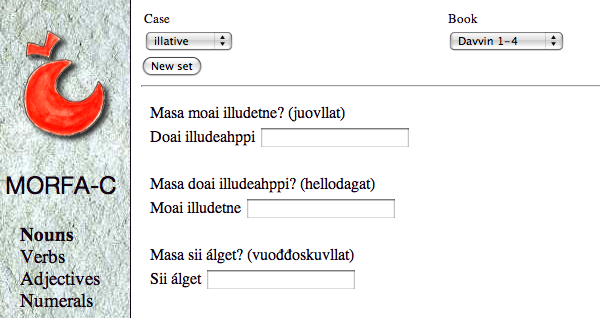
\includegraphics{img/morfaC.png}}
}


%\frame{\frametitle{Morfa-C -- tasks}
%\begin{itemize}
%\item Nouns: nominative pl and all oblique cases (with sg and pl mixed). Also some place names
%\item Verbs: indicative present tense, indicative past tense, conditional, potentional, imperative
%\item Adjectives: grade: positive, comparative and superlative, and as attributive or predicative, all in nominative
%\item Numerals: as attribute in different cases mixed, or as head in nominative pl, accusative, illative, locative and comitative (with sg and pl mixed)
%\end{itemize}
%}


%\frame{\frametitle{Morfa-C -- generating tasks}
%\scalebox{.5}[.5]{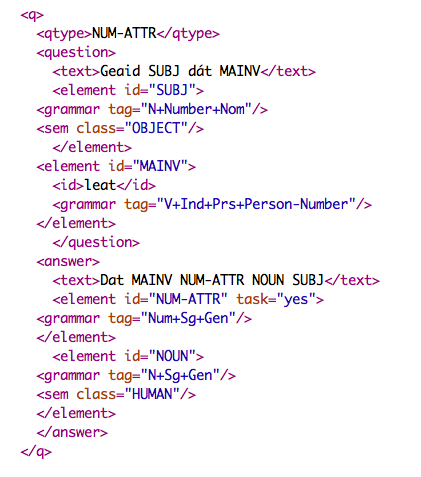
\includegraphics{img/morfa_question.png}}
%}

\frame{\frametitle{Vasta -- open questions}
\scalebox{.5}[.5]{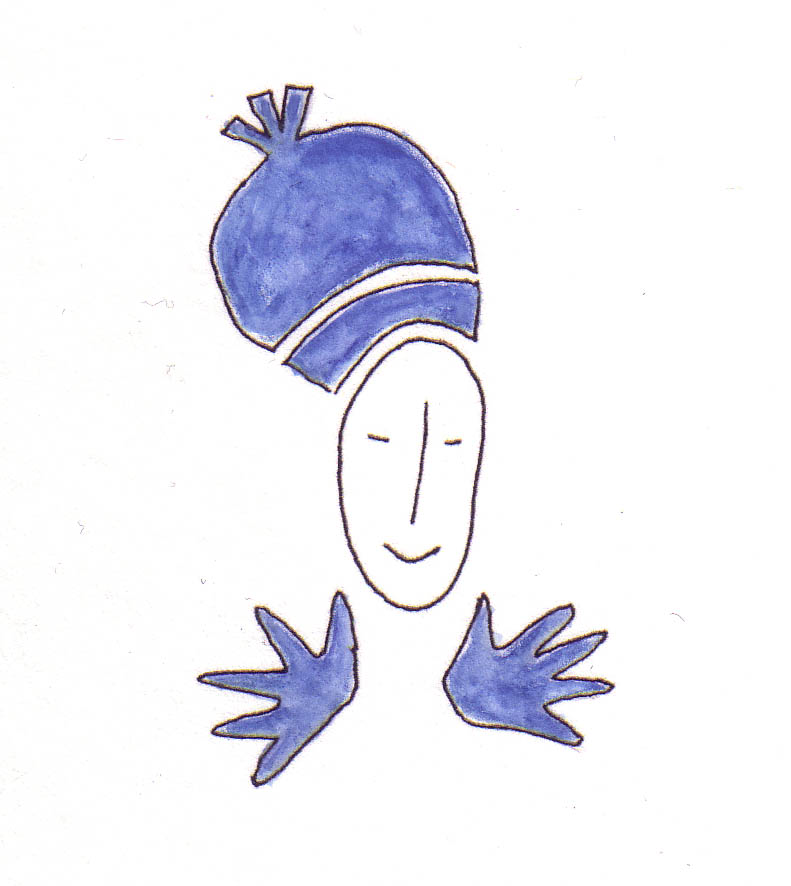
\includegraphics{img/vasta.png}}
}


%\frame{\frametitle{Vasta -- tasks divided into levels}
%\begin{itemize}
%\item Level 1: verb only in present tense, logical cases
%\item  Level 2: verb in past tense, and some verbs with oblique cases, use of postpositions, questions in which the student has to answer with case in plural,  numerals and collective numerals in nominative
%\item  Level 3: grade: numerals inflected in cases, conditional, time expressions, collective numerals
%\end{itemize}
%}



\frame{\frametitle{Sahka -- 7 dialogues}
\scalebox{.55}[.55]{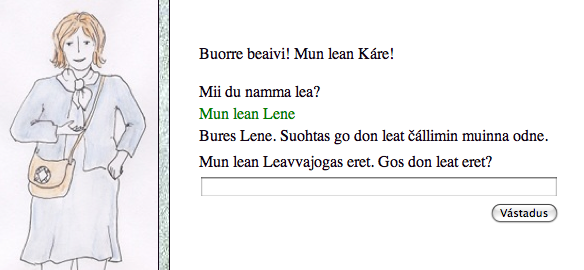
\includegraphics{img/sahka2.png}}\\
}

%\frame{\frametitle{Sahka -- seven dialogues}
%	
%Scenarios:
%\begin{itemize}
%\item Get acquainted to Hánsa -- an adult man living in Kautokeino
%\item Get acquainted to Káre -- an adult woman living in Karasjok
%\item Get acquainted to Lisa -- a girl living in Tana
%\item Get acquainted to Lemet -- a boy living in Tromsø
%\item Visit -- help to move furniture from one room to another, and have a coffee break
%\item Grocery -- buy different kind of food
%\item Comparing in the shop -- tell what is cheapest or most expensive, using adjectives in comparative or superlative
%\end{itemize}
%}

\frame{\frametitle{Sahka -- format}
The comments and questions are tailored, not generated. \\
\vspace{0.5cm}
The dialogue modules:
\begin{itemize}
\item utterance: comment + question: alternative answers link to different utterances/branches
\item topic: opening utterance -- utterances -- closing comment
\item dialogue: opening utterance -- topics -- closing comment
\item small information base: name, place name, car type... 
\end{itemize}
}



\frame{\frametitle{Conclusion}
\begin{itemize}
\item we think we have fulfilled our goals
\item random generation of tasks do that the student can use the programs over and over again
\item reused common LR for other purposes $\rightarrow$ more users
\item maintenance and improvement of common LR will automatically improve OAHPA
\end{itemize}
}

\frame{\frametitle{Future plans}
\begin{itemize}
\item improve the speed of disambiguation
\item improve the feedback system
\item make the programs fully supported in Finnish and English
\item change the main lexicon into xml-format
\item make OAHPA for more Sámi languages -- we have analysers for Lule Sámi (and soon for South Sámi) 
\end{itemize}

}

	
\end{document}

	
